\section{PPO: Proximal Policy Optimization}
Actor-Critic 方法具有 on-policy 性质,需要频繁的交互采样数据,PPO 则通过重要性采样
获得 off-policy 性质从而避免大量的数据采样,同时 PPO 通过裁剪限制策略梯度更新的幅度从而
提高训练的稳定性。

\textbf{重要性采样:}当一个分布的采样困难时,使用另一个分布的采样数据代而计算均值,即
\begin{equation}
    \mathbb{E}_{x\sim p}[f(x)] = \mathbb{E}_{x \sim q}[f(x)\frac{p(x)}{q(x)}],
\end{equation}
但虽均值相同,方差却不同,只有两分布比较接近时,方差才差不多。

在 PPO 中,策略梯度为:
\begin{align}
    \nabla \overline{R}_{\theta} &= \mathbb{E}_{\tau\sim \pi_{\theta}}[R(\tau)\nabla\log\pi_{\theta}(\tau)]\\
    &= \mathbb{E}_{(s_t,a_t)\sim\pi_{\theta}}[A^{\theta}(s_t,a_t)\nabla\log\pi_{\theta}(a_t|s_t)]\\
    &= \mathbb{E}_{(s_t,a_t)\sim\pi_{\theta'}}[\frac{\pi_{\theta}(a_t,s_t)}{\pi_{\theta'}(a_t,s_t)}
    A^{\theta'}(s_t,a_t)\nabla\log\pi_{\theta}(a_t|s_t)]\\
    &= \mathbb{E}_{(s_t,a_t)\sim \pi_{\theta'}}[\frac{\pi_{\theta}(a_t|s_t)}{\pi_{\theta'}(a_t|s_t)}
    A^{\theta'}(s_t,a_t)]\\
    &= J^{\theta'}(\theta),
\end{align}
同时,PPO 的两种优化目标函数分别为:
\begin{align}
    J^{\theta'}_{PPO}(\theta) &= J^{\theta'}(\theta) - \beta KL(\theta' , \theta),\\
    J^{\theta'}_{CLIP PPO}(\theta) &= \mathbb{E}_t[\min(\frac{\pi_{\theta}(a_t|s_t)}{\pi_{\theta'}(a_t|s_t)}A^{\theta'}(s_t,a_t),
    clip(\frac{\pi_{\theta}(a_t|s_t)}{\pi_{\theta'}(a_t|s_t)},1-\epsilon,1+\epsilon)A^{\theta'}(s_t,a_t))].
\end{align}
以上,$\theta'=\theta_{old}$,另外在实际中,还有 critic 网络的训练目标以及熵正则化项等。
在大模型中,通常采用广义优势估计 (GAE),并在每个 token 的奖励中添加一个来自参考模型的 KL 惩罚:
\begin{equation}
    A_t = r(q,o_{\le t}) - \beta \log \frac{\pi_{\theta}(o_t|q,o_{< t})}{\pi_{\theta_{ref}}(o_t|q,o_{< t})} + GAE,
\end{equation}
其中 $r$ 是奖励模型。

\section{GRPO: Group Relative Policy Optimization}
GRPO 与 PPO 类似,但其放弃使用与策略模型大小相当的 critic model,而通过一组评分计算相对优势,
具体为:
\begin{align}
    J_{GRPO}(\theta) &= \mathbb{E}_{q\sim P(Q),\{o_i\}_{i=1}^G\sim \pi_{\theta_{old}}(O|q)}\\
            &\frac{1}{G}\sum_{i=1}^{G}\left(\min(\frac{\pi_{\theta}(o_i|q)}{\pi_{\theta_{old}}(o_i|q)}A_i),
            clip(\frac{\pi_{\theta}(o_i|q)}{\pi_{\theta_{old}}(o_i|q)},1-\epsilon,1+\epsilon)A_i
            -\beta \mathbb{D}_{KL}(\pi_{\theta}||\pi_{\theta_{ref}})\right),\\
            & \quad \mathbb{D}_{KL}(\pi_{\theta}||\pi_{\theta_{ref}}) = \frac{\pi_{ref}(o_i|q)}{\pi_{\theta}(o_i|q)}
            - \log\frac{\pi_{ref}(o_i|q)}{\pi_{\theta}(o_i|q)} -1,
\end{align}
其中每个 $o_i$ 有基于规则的评分 $r_i$,并且优势值的计算为:
\begin{equation}
    A_i = \frac{r_i - mean({r_1,\cdots,r_G})}{std({r_1,\cdots,r_G})}.
\end{equation}

\begin{figure}[H]
    \centering
    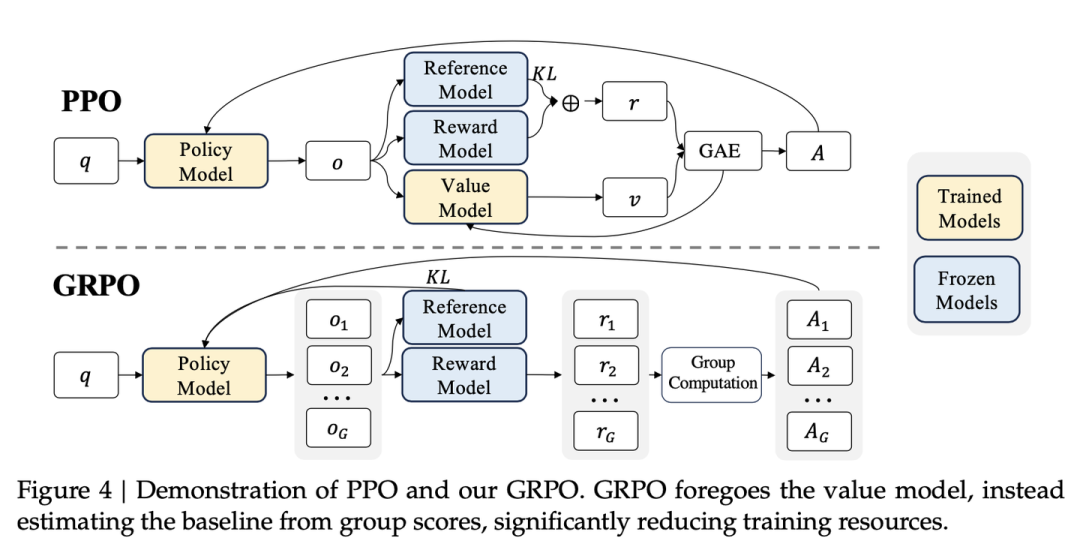
\includegraphics[width=\textwidth]{./fig/PPO GRPO.png}
\end{figure}

